\documentclass[../main.tex]{subfiles}

\begin{document}
\section{Osservabili macroscopici}
Per iniziare a modellizzare il problema del traffico \`e necessario domandarsi quali siano gli osservabili macroscopici principali e come siano legati tra di loro \cite{H111}.
La descrizione di un sistema a livello macroscopico risulta critica ai fini della descrizione della dinamica.
\subsection{Densit\`a}
La densit\`a \`e una variabile tipicamente fisica adotatta nella teoria del traffico.
La densit\`a $\rho$ rappresenta il numero di veicoli per unit\`a di lunghezza della strada.
Sia ora $\Delta x$ la lunghezza di una strada in cui sono presenti $n$ veicoli, allora ad un tempo generico $t$ si ha che
\begin{equation*}
    \rho(n,t,\Delta x)=\frac{n(t)}{\Delta x}
\end{equation*}
La densit\`a si esprime in veicoli al kilometro (veh/km).
Tipicamente per ogni corsia di una strada si ha una $\rho_{max}\sim 10^2$ veh/km.
Si osservi ora come moltiplicando e dividendo per un infinitesimo temporale $dt$ il denominatore divenga l'area dell'intervallo di misura $S$.
In particolare
\begin{equation}
    \rho(t,\Delta x, S)=\frac{n(t)dt}{\Delta x dt}=\frac{\mbox{tempo totale trascorso in }S}{S}
    \label{eq:rho_s}
\end{equation}

\subsection{Flusso}
Il flusso $\Phi$ rappresenta il numero $m$ di veicoli che attraversano un certo localit\`a $x$ in un intervallo di tempo $\Delta t$
\begin{equation}
    \Phi(m, x, \Delta t)=\frac{m}{\Delta t}
\end{equation}
Il flusso \`e espresso in veicoli all'ora (veh/h).
Considerando ora un intorno infinitesimo $dx$ di $x$ \`e possibile ricavare la dipendenza più generale
\begin{equation}
    \Phi(x, \Delta t, S)=\frac{mdx}{\Delta t dx}=\frac{\mbox{distanza totale percorsa dai veicoli in }S}{S}
    \label{eq:phi_s}
\end{equation}

\subsection{Velocit\`a media}
La velocit\`a media \`e definita come il rapporto tra il flusso e la densit\`a: si nota immediatamente come questa non dipenda dall'area dell'intervallo di misura.
Unendo le Eq. (\ref{eq:phi_s}) e (\ref{eq:rho_s}):
\begin{equation}
    \bar{v}(x, t, S)=\frac{\Phi(x, \Delta t, S)}{\rho(t,\Delta x, S)}
\end{equation}
La velocit\`a media \`e espressa in kilometri orari (km/h).
La relazione fondamentale della teoria dei flussi di traffico \`e riassumibile nella:
\begin{equation}
    \Phi=\rho\bar{v}
    \label{eq:fundamental}
\end{equation}

\subsection{Tempo di percorrenza}
Gli osservabili descritti in precedenza, quali velocit\`a media, densit\`a e flusso, sono estremamente utili ai fini di un'analisi quantitativa di un problema di traffico.
Tuttavia, per un problema di questo tipo sarebbe ideale trovare un osservabile il cui valore riesca a far comprendere grossolanamente lo stato del sistema.
Ad esempio, l'informazione fornita dalla frase \emph{la temperatura esterna \`e di circa 27 °C} suggerisce un abbigliamento leggero, mentre l'informazione \emph{la velocit\`a media dell'aria \`e di circa 410 m/s} non \`e molto chiara, pur significando la stessa cosa.
Nel caso del traffico l'osservabile in questione \`e il tempo di percorrenza, definito come il tempo impiegato da un individuo per giungere alla propria destinazione.

Tre diversi andamenti possono essere distinti graficando la frequenza con cui i veicoli impiegano un determinato tempo per percorrere ciascuno il proprio percorso \cite{TravelTime}:
\begin{itemize}
    \item \emph{distribuzione normale unimodale}, tipica di un sistema con densit\`a approssimativamente nulla su ogni strada.
        Tipicamente la gaussiana risultante \`e centrata in prossimit\`a dello zero, o comunque a tempi molto bassi;
    \item \emph{distribuzione lognormale unimodale}, si ottiene caricando il sistema a partire dalla condizione precedente.
        La gaussiana tende ad allungare la coda rivolta verso i tempi pi\`u alti, ad indicare che alcune strade stanno cominciando a congestionarsi;
    \item \emph{distribuzione normale bimodale}, si ottiene una volta giunti alla congestione del sistema.
        In questo caso si hanno due gaussiane con due differenti picchi, rappresentanti veicoli ``fortunati'', che trovano le strade libere, e ``sfortunati'', che rimangono intrappolati in congestione.
\end{itemize}
In Fig. \ref{fig:frequency_distributions} sono rappresentati i tre andamenti, rispettivamente in blu, rosso e verde.
\begin{figure}[H]
    \centering
    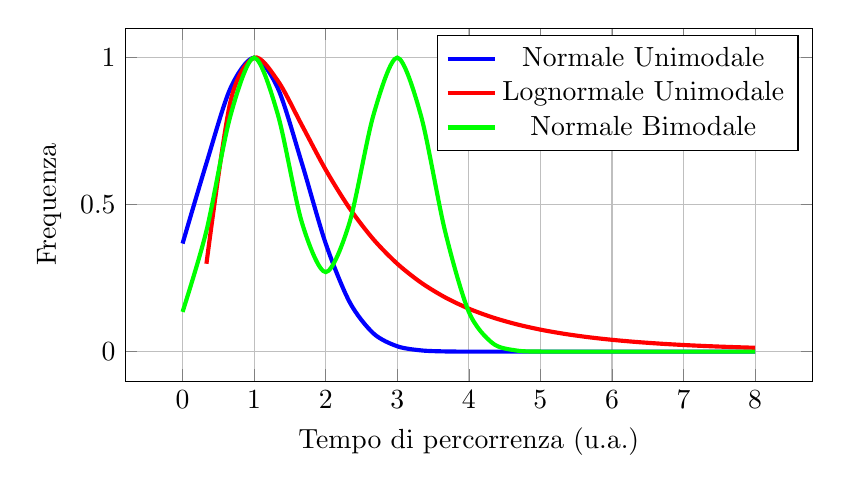
\begin{tikzpicture}
        \begin{axis}[
            grid = both,
            major grid style = {lightgray},
            minor grid style = {lightgray},
            width = 0.85\textwidth,
            height = 0.5\textwidth,
            xlabel = {Tempo di percorrenza (u.a.)},
            ylabel = {Frequenza},]
            \addplot[
                domain = 0:8,
                smooth,
                color = blue,
                line width = 1.5pt,] {e^(-(x-1)^2)};
            \addplot[
                domain = 0:8,
                smooth,
                color = red,
                line width = 1.5pt,] {e^(-ln(x)^2)};
            \addplot[
                domain = 0:8,
                smooth,
                color = green,
                line width = 1.5pt,] {e^(-2*((x-1)^2))+e^(-(2*(x-3)^2))};
        \legend{Normale Unimodale, Lognormale Unimodale, Normale Bimodale}
        \end{axis}
    \end{tikzpicture}
    \caption[Frequenza di veicoli in funzione del tempo di percorrenza]{\emph{Frequenza di veicoli in funzione del tempo di percorrenza. Le curve non sono normalizzate.}}
    \label{fig:frequency_distributions}
\end{figure}

\section{Diagrammi Fondamentali Macroscopici}
A causa della relazione fondamentale del traffico riportata in Eq. (\ref{eq:fundamental}) risulta chiaro come su tre osservabili analizzati si abbiano solamente due variabili indipendenti.
\begin{figure}[H]
\centering
\begin{tikzpicture}[scale=0.5]
    
\begin{groupplot}[group style={group size=2 by 2}]
\nextgroupplot[
    axis y line = left,
    axis x line = bottom,
    ymax = 1.1,
    xmax = 1.1,
    ytick={0.5, 1},
    yticklabels={$\bar{v}_c$,$\bar{v}_l$},
    xtick={0.5, 1},
    xticklabels={$\rho_c$,$\rho_t$}]
\addplot [thick, domain=0:1] {-x+1};
\nextgroupplot[
    axis y line = left,
    axis x line = bottom,
    ymax = 0.823,
    xmin = -1,
    xmax = 0.1,
    ytick={0, 1/1.41},
    yticklabels={$\bar{v}_c$,$\bar{v}_l$},
    xtick={0},
    xticklabels={$\Phi_c$}]
\addplot [samples=200, thick, domain=-1:0] {sqrt(-x/2)};
\addplot [samples=200, thick,  domain=-1:0] {-sqrt(-x/2)};
\nextgroupplot[
    axis y line = left,
    axis x line = bottom,
    ymax = 1.1,
    xmax = 1.1,
    ytick={1},
    yticklabels={$\Phi_c$},
    xtick={0, 1},
    xticklabels={$\rho_c$,$\rho_t$}]
\addplot [samples=200, thick, domain=-1:1] {-x^2+1};
\end{groupplot}

\end{tikzpicture}
\caption[DFM di Greenshield]{\emph{Diagrammi Fondamentali Macroscopici di Greenshield.}}
\label{fig:greenshield}
\end{figure}
In una situazione stazionaria (rete in equilibrio) \`e possibile descrivere il sistema graficamente con tre diagrammi, detti Diagrammi Fondamentali Macroscopici (DFM): $\bar{v}$/$\Phi$, $\Phi$/$\rho$ e $\bar{v}$/$\rho$.
La prima formulazione di questi, riportata come esempio in Fig. \ref{fig:greenshield}, \`e stata effettuata da Greenshield sulla base di alcune misurazioni da lui eseguite.
Assumendo lineare la relazione tra $\rho$ e $\bar{v}$ le relazioni negli altri due diagrammi risultano paraboliche.
In particolare, si ottengono un massimo di flusso sia a $\rho_c=\frac{\rho_t}{2}$ sia per $\bar{v}_c=\frac{\bar{v}_l}{2}$, con $\rho_j$ e $\bar{v}_l$ capacit\`a e velocit\`a massime, rispettivamente.
\\Studiando i diagrammi fondamentali \`e possibile suddividere le condizioni di traffico in tre regimi:
\begin{itemize}
    \item \emph{completamente libero}, quando i veicoli non sono condizionati dal traffico ed \`e per loro possibile viaggiare alla velocit\`a massima $\bar{v}_l$, ossia la velocit\`a \emph{libera}.
        La velocit\`a libera dipende solo dalla geometria e dalle restrizioni applicate ad una strada.
        Si osservi come per questo valore di velocit\`a si abbiano un flusso e una densit\`a prossimi allo $0$.
    \item \emph{saturo}, ove nelle strade sature il flusso e la velocit\`a tendono a $0$ e i veicoli si accodano ad una densit\`a massima $\rho_t$ (densit\`a di \emph{traffico}).
    \item \emph{capacitivo}, in cui la capacit\`a della strada eguaglia il flusso massimo $\Phi_c$, il quale ha associate una densit\`a $\rho_c$ e una velocit\`a $\bar{v}_c$.
        Si ha sempre $\bar{v}_c<\bar{v}_l$.
\end{itemize}

\section{Networks}
In generale, per costruire un qualsiasi modello fisico \`e necessaria una base matematica di partenza.
Nell'ambito degli studi di traffico \`e largamente utilizzata la teoria dei network per rappresentare le reti stradali e lavorare su di esse.

Formalmente, un network \`e descritto da una matrice di adiacenza $\mathcal{A}_{ij}=\left\{0,1\right\}$ in cui la cella $(i,j)$ assume il valore $1$ se il nodo $i$ \`e connesso al nodo $j$, $0$ altrimenti.
Nel caso di network stradali \`e convenzione considerare matrici di adiacenza simmetriche, tali che $\mathcal{A}_{ij}=\mathcal{A}_{ji}$.
Affiancata alla matrice di adiacenza si usa definire spesso la matrice dei pesi $\mathcal{W}_{ij}$, la quale definisce il peso di ciascun collegamento tra nodi.
In particolare, la matrice $\mathcal{W}_{ij}$ possiede le seguenti propiet\`a:
\begin{itemize}
    \item $\mathcal{A}_{ij} = 0 \Longrightarrow \mathcal{W}_{ij} = 0$;
    \item $\mathcal{A}_{ij} = 1 \Longrightarrow \mathcal{W}_{ij} \neq 0$.
\end{itemize}
Dalla matrice di adiacenza \`e possibile definire il grado del nodo $i$-esimo come
\begin{equation*}
    d_i=\sum_j\mathcal{A}_{ij}\\
\end{equation*}
che indica il numero dei link per ogni nodo.
\\Una volta note le matrici di adiacenza e il vettore dei gradi la matrice Laplaciana del network \`e definita come
\begin{equation}
    \mathcal{L}_{ij}=d_i\delta_{ij}-\mathcal{A}_{ij}
\end{equation}
ed ha le seguenti propriet\`a:
\begin{itemize}
    \item \`e semi-definita positiva;
    \item $\mathcal{L}_{ij}>0\Longleftrightarrow i=j$;
    \item $\sum_j\mathcal{L}_{ij}=\sum_i\mathcal{L}_{ij}=0$, quindi esiste un autovalore nullo $\lambda_0$ con corrispondente autovettore $\vec{v}_0=(1,\ldots,1)$;
    \item $\sum_i\mathcal{L}_{ii}=2m$, dove $m$ \`e il numero totale dei link.
\end{itemize}
La presenza di pi\`u autovalori nulli all'interno della matrice Laplaciana evidenzia una disconnessione del network (un approfondimento \`e presente in Appendice \ref{appendix:laplacian}).
In particolare, dati un numero $x$ di autovalori nulli il network \`e separabile in altrettanti subnetwork non connessi tra loro.
\subsection{Random Walk su network}
Si assuma ora che la rete abbia in totale $M$ nodi e che ognuno di essi possa scambiare particelle coi suoi vicini.
Sia $\pi_{ij}$ la matrice stocastica che definisce la probabilità che una particella effettui il viaggio tra nodi $j\to i$.
Questa possiede le seguenti proprietà:
\begin{itemize}
    \item $\mathcal{A}_{ij}=0 \Longrightarrow \pi_{ij}=0$;
    \item $\sum_j\pi_{ij}=1$.
\end{itemize}
Assumendo inoltre di avere $N$ particelle nella rete, \`e possibile definire la funzione $\delta_\alpha(i,t)$ che vale $1$ se la particella $\alpha$ si trova nel nodo $i$ al tempo $t$, 0 altrimenti.
\\Ogni particella segue quindi la dinamica
\begin{equation*}
    \delta_\alpha(i,t+\Delta t)=\sum_j\xi_{ij}^\alpha\delta_\alpha(j,t)
\end{equation*}
dove $\xi_{ij}^\alpha$ \`e una matrice random che prende valori della base standard $\widehat{e}_i\in \mathbb{R}^M$ con probabilità $\pi_{ij}$.
Il numero di particelle nel nodo $i$ al tempo $t$ \`e dato da
\begin{equation*}
    n_i(t)=\sum_\alpha\delta_\alpha(i,t)
\end{equation*}
ed \`e possibile dimostrare \cite{RandomWalks} che la seguente equazione \`e un integrale del moto
\begin{equation}
    \sum_in_i(t)=N
\end{equation}

\end{document}